\documentclass[conference]{IEEEtran}
\usepackage{graphicx}
\usepackage{booktabs}
\usepackage{array}
\usepackage{url}
\usepackage[hidelinks]{hyperref}
\usepackage{listings}
\lstset{basicstyle=\ttfamily\footnotesize,columns=fullflexible,breaklines=true,frame=single,xleftmargin=2pt,xrightmargin=2pt}
\newcommand{\cmd}[1]{\texttt{#1}}

\begin{document}

\title{Hardening a Two-Host Private Service Network:\\ Backup DNS, TTL-Driven Cutover, Service Isolation and Edge Failover}

\author{\IEEEauthorblockN{Yatin Singh}
\IEEEauthorblockA{\textit{B.Tech CS \& AI}\\
\textit{Newton School of Technology}\\
\textit{Rishihood University}}
\and
\IEEEauthorblockN{Dadi Dinesh}
\IEEEauthorblockA{\textit{B.Tech CS \& AI}\\
\textit{Newton School of Technology}\\
\textit{Rishihood University}}}

\maketitle

\begin{abstract}
This report describes Phase~2 of a Computer Networks course project in which a private service network was built by hand on two macOS laptops connected to one Wi-Fi hotspot. In Phase~1 a client resolved the private name \cmd{app.team1.test} through a dnsmasq resolver, connected over HTTPS to an nginx edge that terminates TLS with a locally issued certificate, and was load-balanced across two Express backends. Phase~2 extends this system with five resilience mechanisms: a backup DNS resolver, a controlled record change governed by a 30-second TTL, packet-filter isolation of the backend ports, passive health-check failover in nginx, and a DNS-based migration to a standby edge. Each mechanism was demonstrated with a before/after test. We also report the faults met while running the tests and the layer-by-layer method used to diagnose them. The results show that each mechanism works as intended, and that the edge host remains the single point of failure of the design.
\end{abstract}

\begin{IEEEkeywords}
DNS, TTL, dnsmasq, nginx, load balancing, failover, TLS termination, packet filter, troubleshooting
\end{IEEEkeywords}

\section{Introduction}
A request to a web service crosses several independent layers: name resolution, IP reachability, a TCP connection, a TLS handshake and finally the HTTP exchange. Phase~1 of the project built each of these layers on two laptops and captured them with Wireshark. Phase~2 asks a different question: what happens when a part of the system fails or has to change, and how can the network be made to tolerate it?

The brief defines six extensions: (A) a backup DNS resolver, (B) TTL and a controlled record change, (C) isolation of the backend services, (D) high-availability failover, (E) a DNS-based edge migration and (F) a faculty-injected troubleshooting challenge. This report documents the design of A--E, the tests used to demonstrate them, the faults encountered and the lessons learned. Extension~F is evaluated live; Section~\ref{sec:trouble} describes the diagnostic method we use for it.

\section{System Architecture}
\subsection{Machines and Roles}
The team has two members and therefore two laptops; the brief allows teams of two or three to combine machine roles. Table~\ref{tab:roles} lists the roles. Mac~1 is a college-managed laptop whose application firewall blocks incoming LAN connections and cannot be changed by the user. During Phase~1 we confirmed this with \cmd{tcpdump}: DNS queries reached the host but no reply left it, while queries to its loopback address were answered. Mac~1 therefore acts as the client, and every server role runs on Mac~2.

\begin{table}[htbp]
\caption{Machine Roles and Services}
\label{tab:roles}
\centering
\begin{tabular}{@{}l l l@{}}
\toprule
Host & Role & Service / port \\
\midrule
Mac 1 & Client & browser, curl, dig, Wireshark \\
Mac 2 & DNS & dnsmasq, UDP 53 \\
Mac 2 & Edge & nginx, TCP 443 (80 $\rightarrow$ 301) \\
Mac 2 & Backend A & Express, TCP 4000 \\
Mac 2 & Backend B & Express, TCP 6000 \\
\midrule
\multicolumn{3}{@{}l@{}}{\textit{Added in Phase 2 (loopback of Mac 1):}}\\
Mac 1 & Backup DNS & dnsmasq, 127.0.0.1:53 \\
Mac 1 & Standby edge & nginx, 127.0.0.1:443 \\
\bottomrule
\end{tabular}
\end{table}

\subsection{Request Path}
Fig.~\ref{fig:topo} shows the topology and request flow. The client queries dnsmasq for \cmd{app.team1.test}, which answers with Mac~2's address. The client opens a TCP connection to port 443 and completes a TLS handshake; the certificate carries \cmd{app.team1.test} and \cmd{api.team1.test} as Subject Alternative Names and is signed by a local certificate authority (``Team1 Local CA'') that the client trusts. nginx terminates TLS and forwards plain HTTP over loopback to one of the two backends in round-robin order. The \cmd{.test} top-level domain is reserved~\cite{rfc6761}, so public resolvers return NXDOMAIN for it and it cannot clash with a real name.

\begin{figure}[htbp]
\centerline{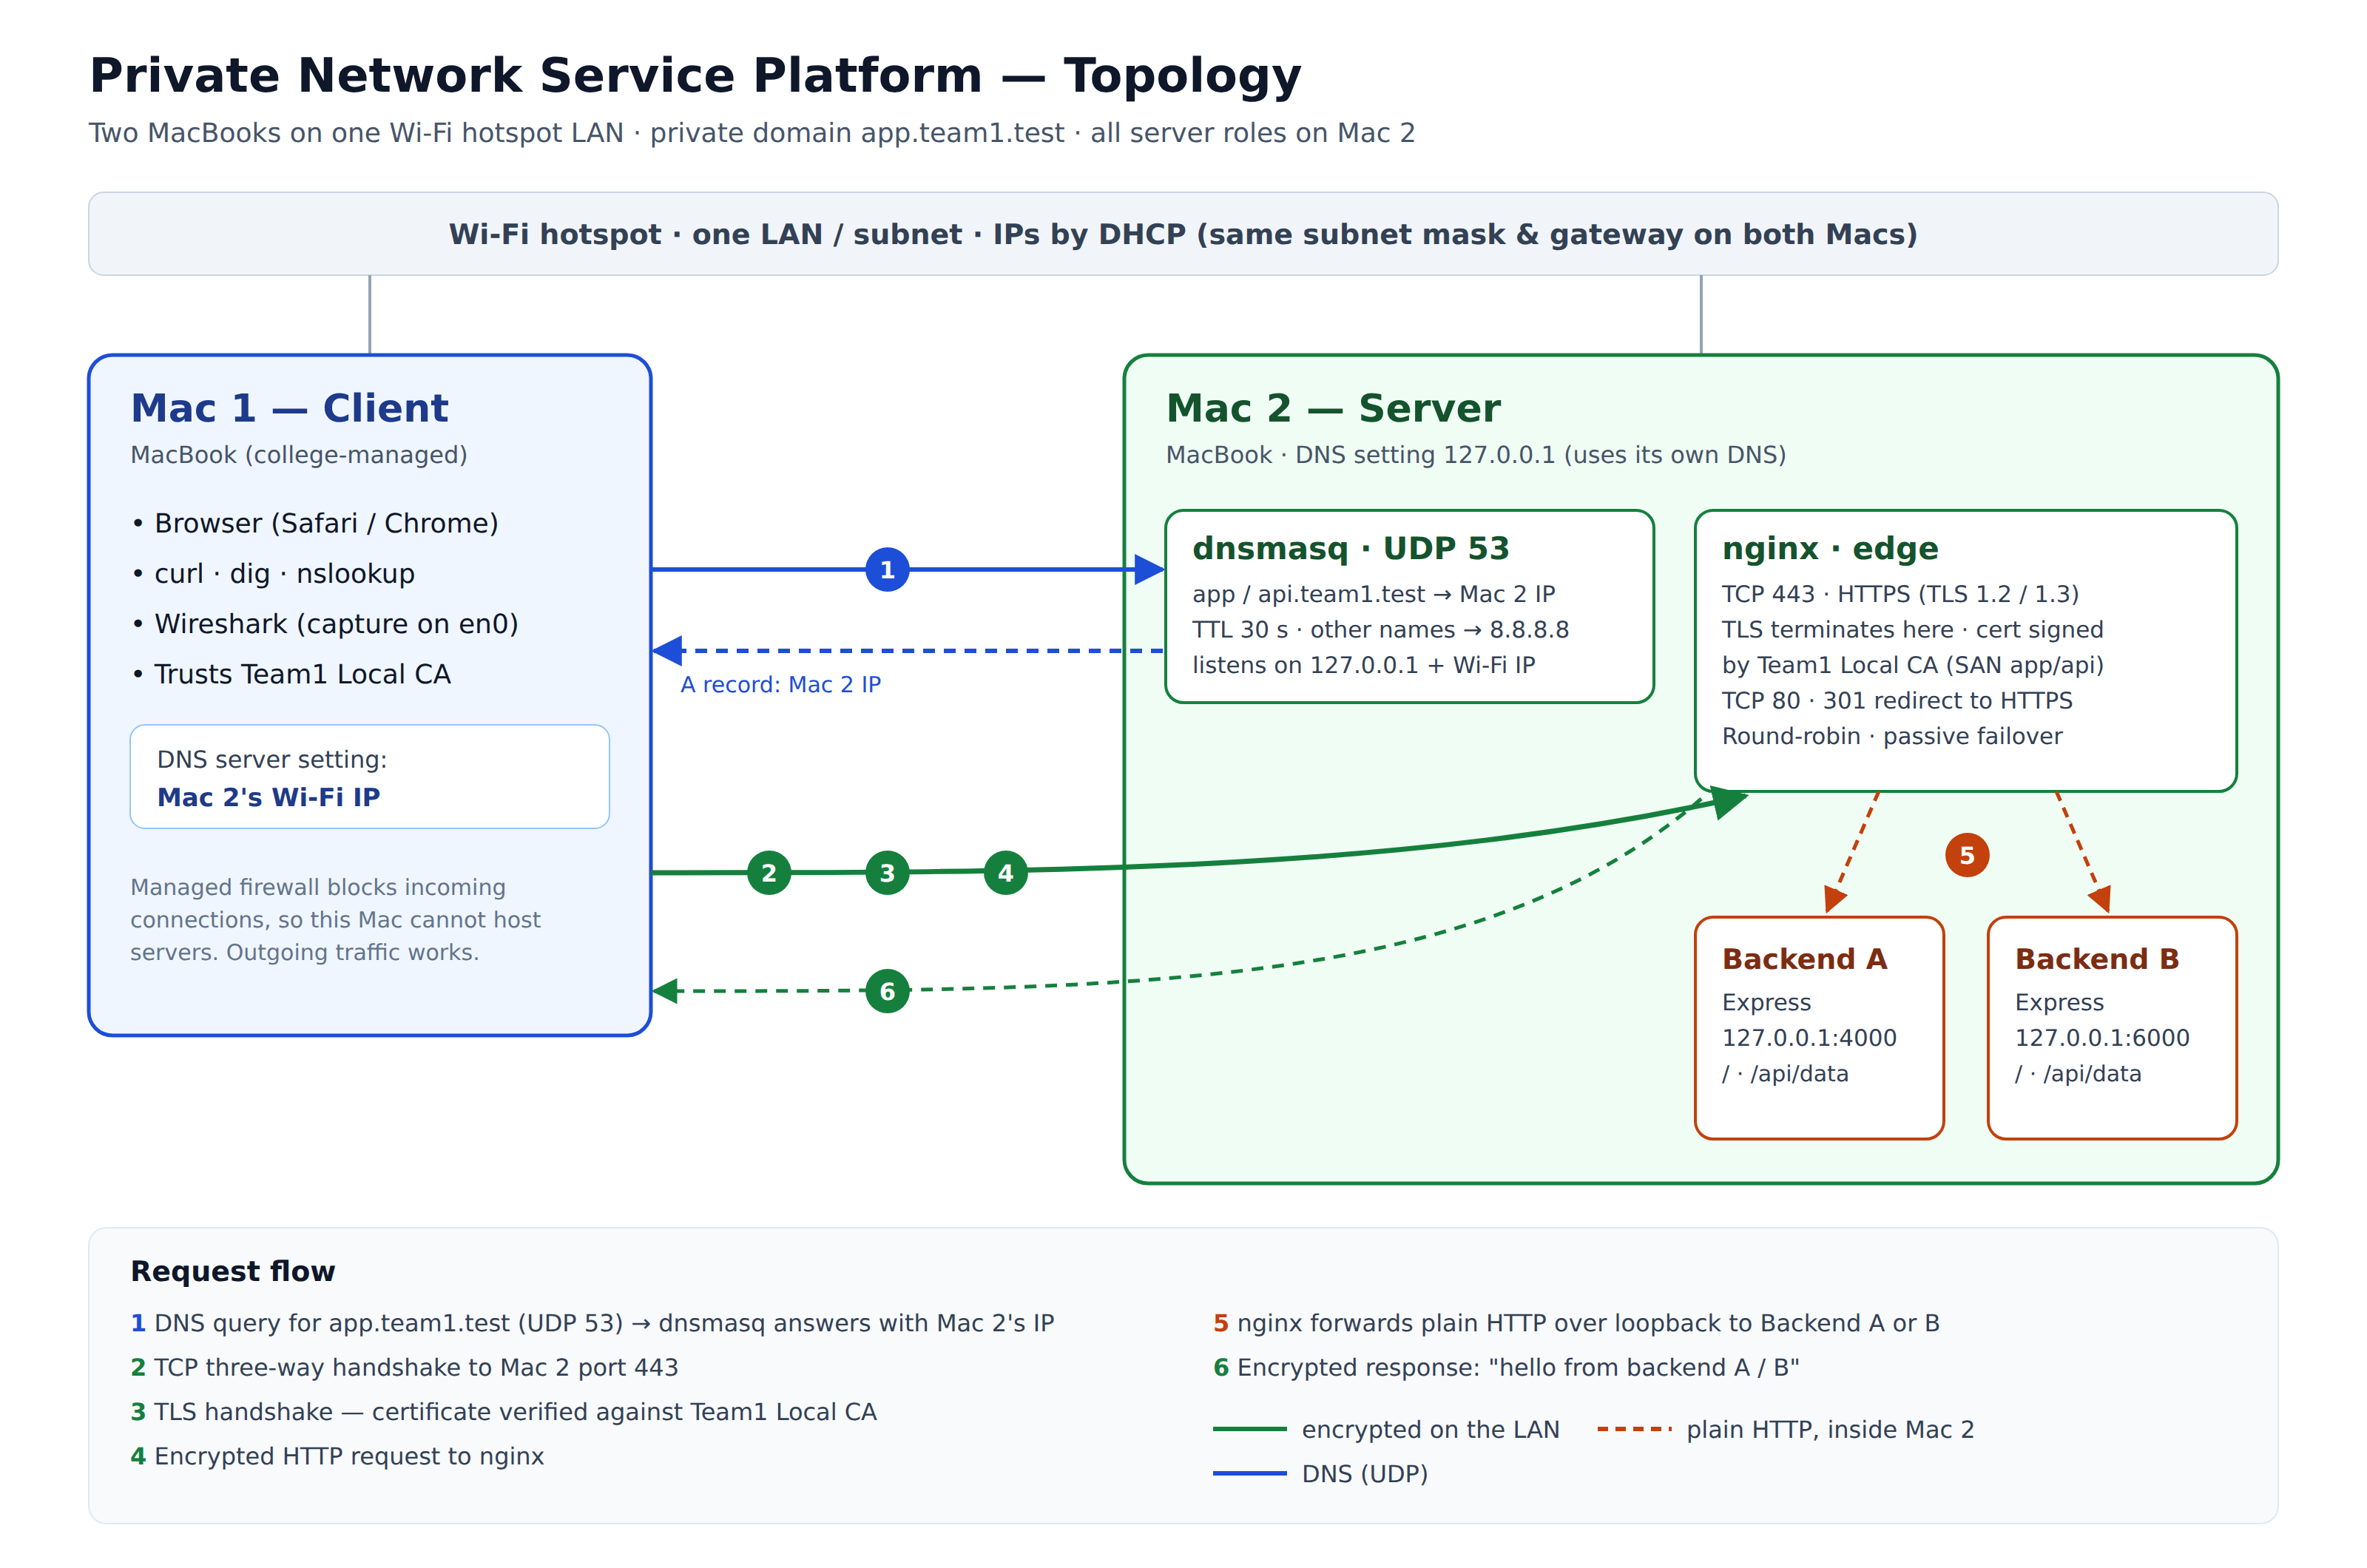
\includegraphics[width=\columnwidth]{topology.png}}
\caption{Topology and request flow. Steps 1--6: DNS query, TCP handshake, TLS handshake, encrypted request, plain HTTP to a backend, encrypted response.}
\label{fig:topo}
\end{figure}

\section{Phase 2 Extensions}
Because Mac~1 cannot accept LAN connections, the backup resolver (A) and the standby edge (E) run on Mac~1's loopback interface and serve Mac~1 itself, which is the client in every test. The mechanisms being demonstrated---resolver fallback and TTL-governed cutover---behave the same way as they would on a separate host.

\subsection{Backup DNS Resolver (Extension A)}
\textit{Design.} A second dnsmasq~\cite{dnsmasq} instance on Mac~1 listens on 127.0.0.1 and holds the same \cmd{address=} records as the primary, both pointing to Mac~2. The client's resolver list is set to the primary (Mac~2) followed by the backup (127.0.0.1).

\textit{Test.} With both resolvers running, names resolved through the primary. The primary was then stopped with \cmd{brew services stop dnsmasq} on Mac~2.

\textit{Result.} Mac~1 continued to resolve \cmd{app.team1.test} to Mac~2's address; \cmd{dig} reported \cmd{SERVER: 127.0.0.1\#53}, and \cmd{https://app.team1.test} kept loading. A DNS failure differs from an application failure: in the first the client cannot obtain an address and never contacts the server (NXDOMAIN or a timeout); in the second resolution succeeds but the server returns an error, such as nginx's \cmd{502 Bad Gateway} when no backend is available.

\subsection{TTL and Controlled Record Change (Extension B)}
\textit{Design.} The project records carry \cmd{local-ttl=30}, so every answer may be cached for 30 seconds~\cite{rfc1034}.

\textit{Test.} The name was resolved on Mac~1 with \cmd{dscacheutil}, which reads the operating-system cache. The record on Mac~2 was then changed to 10.10.10.10 and dnsmasq restarted, and the lookup was repeated every ten seconds.

\textit{Result.} Mac~1 kept returning the cached address until the TTL expired and then returned 10.10.10.10. After the record was restored, flushing the cache (\cmd{dscacheutil -flushcache}, \cmd{killall -HUP mDNSResponder}) made the change visible at once. \cmd{dig} is unsuitable for this test because it queries the server directly and bypasses the cache. In production, operators lower the TTL before a migration so that a record change propagates in seconds rather than hours, and keep the old target running until cached answers expire.

\subsection{Service Isolation (Extension C)}
\textit{Design.} Before Phase~2 the backends listened on all interfaces, so a client could bypass the edge. We added a pf~\cite{pf} rule on Mac~2, after backing up \cmd{/etc/pf.conf}:
\begin{lstlisting}
set skip on lo0
block drop in quick on en0 proto tcp \
      from any to any port { 4000 6000 }
pass all
\end{lstlisting}

\textit{Result.} Before the rule, \cmd{curl http://<Mac 2>:4000} from Mac~1 reached Backend~A directly; afterwards the same request timed out, while \cmd{https://app.team1.test} still worked because nginx reaches the backends over the skipped loopback interface. The original ruleset was restored with \cmd{pfctl -f /etc/pf.conf}; pf had been enabled by the system before the demonstration, so it was left enabled. Our backend ports are 4000 and 6000 rather than the brief's 3001 and 3002; the isolation logic is unchanged.

\subsection{High-Availability Failover (Extension D)}
\textit{Design.} Each upstream server is declared with \cmd{max\_fails=1 fail\_timeout=10s}, and \cmd{proxy\_next\_upstream error timeout http\_502 http\_503} lets nginx retry a failed attempt on the other server~\cite{nginxup}. This is passive health checking: a backend is marked unavailable after a real request to it fails.

\textit{Test and result.} Six consecutive requests alternated between Backends A and B. With Backend~A stopped, all six were served by Backend~B and none failed. After Backend~A was restarted and \cmd{fail\_timeout} elapsed, requests alternated again.

\textit{Single point of failure.} Mac~2 still hosts the resolver, the edge and both backends; if it fails the service is unavailable. Removing this requires a second edge on another host sharing a floating virtual IP (e.g., VRRP via keepalived) or DNS failover across two edges, and backends on separate hosts.

\subsection{DNS-Based Edge Cutover (Extension E)}
\textit{Design.} A standby nginx on Mac~1 uses the same certificate and the same upstream servers. Each edge adds a response header identifying itself (\cmd{X-Edge: mac2} or \cmd{X-Edge: mac1}).

\textit{Test.} A loop on Mac~1 requested \cmd{https://app.team1.test} every five seconds and printed the header. On Mac~2 the \cmd{app.team1.test} record was changed to point to the standby edge and dnsmasq restarted.

\textit{Result.} Responses kept arriving from \cmd{mac2} for up to 30~seconds, while the cached answer was valid, and then switched to \cmd{mac1}. No certificate warning appeared, because both edges present the same certificate for the same name~\cite{rfc8446}. The record was then restored.

\section{Troubleshooting Findings}\label{sec:trouble}
Table~\ref{tab:faults} lists the faults met while running the tests. All of them presented as ``the site does not load'', yet four of the five were at the DNS layer.

\begin{table*}[htbp]
\caption{Faults Encountered and Their Diagnosis}
\label{tab:faults}
\centering
\begin{tabular}{@{}>{\raggedright}p{4.2cm} l >{\raggedright}p{5.6cm} >{\raggedright\arraybackslash}p{4.6cm}@{}}
\toprule
Symptom & Layer & Cause & Fix \\
\midrule
\cmd{dig} on Mac 1 returned NXDOMAIN from an IPv6 server & DNS & Hotspot also advertised an IPv6 resolver, which was queried first and does not know \cmd{.test} & Disabled IPv6 on the client during testing \\
Queries to Mac 2 timed out after changing hotspot & IP / DNS & New DHCP address; dnsmasq still bound to the old one & Rewrote \cmd{listen-address} and records with the current IP \\
Port 53 on Mac 2 held by Cloudflare WARP & DNS & WARP DNS proxy running; dnsmasq not running & Disconnected WARP, restarted dnsmasq, checked \cmd{lsof -iUDP:53} \\
Backup resolver never answered & DNS & Config contained a literal placeholder instead of an IP, so dnsmasq failed to start & Rewrote config with the real address \\
curl reported \cmd{dns:0 connect:0} & DNS & Resolution failed before any connection; \cmd{curl -v} showed a resolver timeout & Queried each resolver with \cmd{dig @server} to isolate the faulty one \\
\bottomrule
\end{tabular}
\end{table*}

The method we use for these faults and for Extension~F checks one layer at a time, bottom-up: name resolution (\cmd{dig}), IP reachability (\cmd{ping}), TCP (\cmd{nc -vz host 443}), TLS (\cmd{openssl s\_client}), HTTP (\cmd{curl -v}) and finally the nginx error log, which names a failing upstream. A \cmd{502} at the last step points to the backends, not the network.

\section{Discussion}
The extensions fall into two groups. A, D and E add redundancy, but each moves the single point of failure rather than removing it: the backup resolver and the standby edge share a host with the client, and the primary edge shares a host with every other server. B and E show that DNS-based traffic management is bounded by caching: the TTL is a trade-off between query load and how quickly a change takes effect. C shows that placing services behind a reverse proxy is not by itself isolation; the ports must also be closed on the network interface. A practical constraint was the managed client laptop, which could host services only on its loopback interface; with a third unmanaged host, the backup resolver and standby edge would serve every client on the LAN.

\section{Conclusion}
Building on the Phase~1 network, we demonstrated a backup resolver that keeps names resolvable when the primary stops, TTL-governed propagation of a record change, firewall isolation that leaves only the edge able to reach the backends, automatic failover and recovery in nginx, and a DNS-based migration to a standby edge. Each test confirmed the expected behaviour. The remaining single point of failure is the edge host, which a floating virtual IP shared by two edges would remove.

\begin{thebibliography}{00}
\bibitem{rfc1034} P. Mockapetris, ``Domain names---concepts and facilities,'' RFC 1034, IETF, Nov. 1987.
\bibitem{rfc6761} S. Cheshire and M. Krochmal, ``Special-use domain names,'' RFC 6761, IETF, Feb. 2013.
\bibitem{rfc8446} E. Rescorla, ``The Transport Layer Security (TLS) protocol version 1.3,'' RFC 8446, IETF, Aug. 2018.
\bibitem{nginxup} NGINX, ``Module ngx\_http\_upstream\_module,'' nginx documentation. [Online]. Available: \url{https://nginx.org/en/docs/http/ngx_http_upstream_module.html}
\bibitem{dnsmasq} S. Kelley, ``dnsmasq,'' manual page. [Online]. Available: \url{https://thekelleys.org.uk/dnsmasq/docs/dnsmasq-man.html}
\bibitem{pf} OpenBSD, ``pf.conf---packet filter configuration file,'' manual page. [Online]. Available: \url{https://man.openbsd.org/pf.conf}
\end{thebibliography}

\end{document}
